\documentclass[12pt]{extarticle}

\usepackage{preamble}
\usepackage{bytefield}
\usepackage{minted}

\title{Computer Science 2 Notes, Partial 2}
\date{Semester 2, 2023/2024}

\setlength{\headheight}{15pt} % ??? we do what fancyhdr tells us to do

\begin{document}

\maketitle
\tableofcontents
\clearpage

% Class of 20/03/2024
\section{Dynamic programming}

This is a general technique to constructing algorithms, it is not a specific solution to a specific problem but a way to think about problems.

\subsection{Shortest path in DAGs}

We saw this problem before but now we will approach it in a different way.

In unweighted graphs we used BFS to compute the path from a \textit{single source} to all the other vertices and takes $\O(|V| + |E|)$, while in weighted graphs we used Dijkstra's algorithm which also works for \textit{single source} shortest path and takes $\O(|E| \log |V|)$ when implemented using fibonacci heaps.

But if we know that the graph is acyclic we can do better: nodes are removed from the queue in a topological order, then we can write the following algorithm:

\begin{minted}{python}
    def shortest_path_dag(G, cost, s):
        d = {}
        for v in G.vertices():
            d[v] = float('inf')

        # Calculate the topological sort
        topological_sort = topological_sort(G)

        # We will only be able to explore the nodes that
        # come after s in the topological sort
        index_of_s = topological_sort.index(s)
        topological_sort = topological_sort[index_of_s:]

        # The distance of the starting node to itself is 0
        d[s] = 0

        # We iterate in topological order
        for u in topological_sort:

            # We check all the neighbors of v
            for v in u.neighbors():
                # If the cost of getting to v from u is less than
                # the current cost of getting to v, we update it
                
                d[u] = min(d[u], d[v] + cost((u, v)))

        return d
\end{minted}

Note that this algorithm works only for acyclic graphs, but also in the case of negative weights.

\subsubsection{Time complexity}

We saw before that the time complexity of the topological sort is $\O(|V| + |E|)$, the loop is also $\O(|V| + |E|)$, therefore the total time complexity is $\O(|V| + |E|)$.

Moreover the space complexity is $\O(|V|)$ because we need to store the distances from the source to all the other nodes.

There is really no way to optimize this further, at least on a theoretical level.

\subsubsection{Longest path on DAGs}

We can solve this problem in the same way as the shortest path problem but we negate the cost of the edges.

In this way the longest path problem becomes a shortest path problem and we can use the same algorithm.

Alternatively we could replace the \texttt{min} with a \texttt{max} in the algorithm and get the same result.

\subsubsection{Adding a sink to the graph}

Consider a DAG where we know already the distances from a starting node to all the other nodes, and we want to add a sink $v$ to the graph.

We create edges $(u_i, v)$ where $u_i$ are the nodes that are already in the graph that we connect to $v$, then we add $v$ to the topological sort as the last element (since it is a sink).

Now we can compute the shortest path from the source to $v$ by iterating all the $u_i$ and choosing the one such that $d[u_i] + c(u_i, v)$ is the smallest.

We can use this method to create a new algorithm where we add each node to the graph one by one and compute the shortest path to the new node.

\begin{minted}{python}
    def shortest_path_dag(G, cost, s):
        # The setup is the same as before

        d = {}
        for v in G.vertices():
            d[v] = float('inf')

        topological_sort = topological_sort(G)
        index_of_s = topological_sort.index(s)
        topological_sort = topological_sort[index_of_s:]

        d[s] = 0

        for u in topological_sort:
            for v in u.neighbors():
                d[u] = min(d[u], d[v] + cost((v, u)))

\end{minted}

\subsection{The knapsack problem}

\subsubsection{The problem}

In this problem we have a set of $n$ items, each with a weight $w_i$ and a value $v_i$, and we have to put them in a backpack with a maximum capacity $W$.

The problem is to find the best combination of items that maximizes the value of the backpack.

\subsubsection{Example}

Suppose we have a maximum weight $W = 20$ and the following items

\begin{table}[H]
    \centering
    \begin{tabular}{ |c|c|c|c|c| }
        \hline
        \textbf{Item}   & 1  & 2  & 3 & 4  \\
        \hline
        \textbf{Value}  & 4  & 7  & 1 & 5  \\
        \textbf{Weight} & 10 & 12 & 9 & 10 \\
        \hline
    \end{tabular}

    \label{tab:knapsack_example}
    \caption{An example set of items}
\end{table}

Then the solution is to take item 1 and item 4, which have a total weight of 20 and a total value of 9.

As we can see this problem cannot be solved using a greedy algorithm, because such an algorithm would choose item 2 first and then stop because we are already at the maximum weight.

\subsubsection{Recursive formulation}

Consider the situation where we have a backpack with a maximum weight $W$ and a set of $n$ items $I$.

We already have the solution for the problem with $n-1$ items provided as a function $f : [0, W] \in \N \to A \subseteq I$ that maps the maximum weight of the backpack to the set of items that we can put in the backpack.

Now we consider the $n$-th item, we have two possibilities: either we take it or we don't.
\begin{itemize}
    \item If we don't take it we already have the best solution, that is $f(W)$.
    \item If we take it, the weight we have left in the backpack is $W - w_n$, therefore the best solution is $f(W - w_n) \cup \{n\}$.
\end{itemize}

We can now write a matrix $M$ of size $(n + 1) \times (W + 1)$ where $M_{ij}$ is the maximum value that we can get with the first $i$ items and a maximum weight of $j$.

We note that in the first row of the matrix we will always have 0, because if we have 0 items we can't have any value.

Moreover we note that when we choose whether to take the $i$-th item or not we have to check if the $w_i$ is greater than the maximum weight we have left, if it is we can't take it.
In particular, in the first column of the matrix we will always have 0, because if we have 0 weight we can't have any value.

At last, note that the to compute $M_{ij}$ we need to know $M_{i-1, j}$ and $M_{i-1, j - w_i}$ which are both values that come before $M_{ij}$ in the matrix.
Therefore we can compute the matrix row by row, from left to right and be sure that we have already computed the values we need.

\subsubsection{The algorithm}

We can now use the recursive definition to formalize the algorithm.

\begin{minted}{python}
    def knapsack(W, I):
        # Initialize the matrix with all 0s
        M = [[0 for _ in range(W + 1)] for _ in range(len(I) + 1)]

        # The iteration starts from 1 because the first row is all 0s
        for i in range(1, len(I) + 1):
            item = I[i - 1]

            # Same as before, we start from 1 because the 
            # first column is all 0s
            for max_weight in range(1, W + 1):
                # If the item is too heavy we can't take it
                # and we just copy the previous value
                if item.weight > max_weight:
                    M[i][max_weight] = M[i - 1][max_weight]
                else:
                    # Otherwise we need to choose the maximum
                    # value between:
                    # - The value of the previous item
                    # - The value of the current item plus
                    #   the value of the best solution for
                    #   the remaining weight
                    M[i][max_weight] = max(
                        M[i - 1][max_weight],
                        M[i - 1][max_weight - item.weight] + item.value
                    )

        return reconstruct(W, I, M)
\end{minted}

Now that we computed the matrix we need to reconstruct the solution, that is, the set of items that we put in the backpack.

\begin{minted}{python}
    def reconstruct(W, I, M):
        solution = []
        weight = W

        # Iterate the rows of the matrix in reverse order
        for i in range(len(I), 1, -1):
            # If the value of the last item of the current row
            # is different from the one of the previous row
            # it means that we took the (i-1)-th item
            if M[i][weight] != M[i - 1][weight]:
                solution.append(I[i - 1])

                # Reduce the weight that we are left with
                # for the next iteration
                weight -= I[i - 1].weight
        
        return solution
\end{minted}

% Class of 21/03/2024

\begin{remark}
    In class we covered also a slight variation of this algorithm that uses recursion but the idea is the same and I think that this formulation is more clear.
    Moreover the recursive function that was presented in class is a \emph{tail recursive function}, therefore it can be easily transformed into a loop like the one presented here.
\end{remark}

\subsection{Edit distance}

The edit distance is a way to measure the difference between two strings.

We define three operations:
\begin{enumerate}
    \item Insertion
    \item Deletion
    \item Substitution
\end{enumerate}

Given two strings $A, B$ we want to find the minimum number of operations to transform $A$ into $B$.

Consider two strings such that $\abs{A}, \abs{B} \leq n$ and the function \texttt{ed} that computes the edit distance between two strings.

We can translate the three operations into a recursive formulation:

\begin{align}
    \texttt{ed}(A, B) & \leq \texttt{ed}(A[0:n-1], B) + 1                                                      \\
    \texttt{ed}(A, B) & \leq \texttt{ed}(A, B[0:n-1]) + 1                                                      \\
    \texttt{ed}(A, B) & \leq \texttt{ed}(A[0:n-1], B[0:n-1]) + (0 \text{ if } A[n-1] = B[n-1] \text{ else } 1)
\end{align}

where the first one is deletion, the second one is insertion and the third one is substitution.
Now we note that the $\texttt{ed}(A, B)$ is the minimum of the three values above.

We can use this to write a recursive algorithm to compute the edit distance.

\subsubsection{The algorithm}

The idea is that we can compute a matrix $M$ of the various edit distances between the substrings of $A$ and $B$: each element $M_{ij}$ is the edit distance between $A[0:i]$ and $B[0:j]$.

Moreover we note that the first row and the first column of the matrix are just the numbers from 0 to the length of the string, because the difference between an empty string and a string of length $i$ is $i$.

\begin{minted}{python}
    def edit_distance(A, B):
        # Initialize the matrix with all 0s
        M = [[0 for _ in range(len(B))] for _ in range(len(A))]

        for i in range(len(A)):
            for j in range(len(B)):
                if i == 0:
                    # The difference between an empty string
                    # and a string of length j is j
                    M[i][j] = j
                elif j == 0:
                    # Same as before, the difference between
                    # a string of length i and an empty string is i
                    M[i][j] = i
                else:
                    # We use the formulas we found before and
                    # we take the minimum value
                    M[i][j] = min(
                        M[i - 1][j] + 1,
                        M[i][j - 1] + 1,
                        M[i - 1][j - 1] +
                            (0 if A[i - 1] == B[j - 1] else 1)
                    )
        return reconstruct(A, B, M)
\end{minted}

As in the previous algorithm we need to reconstruct the solution from the matrix, that is, to find the sequence of operations that transform $A$ into $B$.

\begin{minted}{python}
    def reconstruct(A, B, M):
        solution = []
        i, j = len(A) - 1, len(B) - 1

        while i > 0 and j > 0:
            # If the value of the current cell is the same as 
            # the one of the cell above it means that we 
            # deleted a character
            if M[i][j] == M[i - 1][j] + 1:
                solution.append(f"Delete {A[i]}")
                i -= 1
            # If the value of the current cell is the same as 
            # the one of the cell on the left it means that
            # we inserted a character
            elif M[i][j] == M[i][j - 1] + 1:
                solution.append(f"Insert {B[j]}")
                j -= 1
            # If the value of the current cell is the same as
            # the one of the cell on the top left it means 
            # that we substituted a character
            elif M[i][j] == M[i - 1][j - 1] + 1:
                solution.append(f"Substitute {A[i]} with {B[j]}")
                i -= 1
                j -= 1
            else:
                # If the value of the current cell is the 
                # same as the one of the cell on the top left
                # it means that we didn't do anything
                i -= 1
                j -= 1

\end{minted}

\subsubsection{Time complexity}

We have $n \times n$ subproblems and each subproblem takes $\O(1)$ to compute, therefore the time complexity is $\O(n^2)$.

Moreover the space complexity is also $\O(n^2)$, because that's the size of the matrix.

Note that this is a very expensive algorithm in terms of computational cost. If we consider binary strings and assume each character takes 1 bit, the table would be $4 n^2 $ bytes, which for an input of $n \approx 10^5$ would be $4 \times 10^{10}$ bytes, which is 40 GB.
Time complexity is also very high but usually the limiting factor of this algorithm is the space complexity.

\subsubsection{Optimization}

Note that to compute the $i$-th row we only need the $i-1$-th row and the $i$-th row itself.
Therefore we can store just two rows of the matrix, one for the even indices and one for the odd indices.

In this way we reduced the memory complexity to $\O(n)$ but we lost the information about the sequence of operations that transform $A$ into $B$, we get just the edit distance as a number.

\begin{remark}
    There exists an algorithm that computes the edit distance in $\O(n^2)$ time and $\O(n)$ space and is able to reconstruct the sequence of operations. This is called \emph{Hirschberg's algorithm} but it is quite complex and we won't cover it in this course.
\end{remark}

% Class of 22/03/2024
\subsection{Floyd-Warshall algorithm}

This algorithm is used to compute the shortest path between all pairs of vertices in a graph.

Let the input be the $n \times n$ matrix $A$ where $A_{ij}$ is the weight of the edge between $i$ and $j$ if it exists, otherwise it is $\infty$.

\begin{minted}{python}
    def floyd_warshall(A):
        D = A
        for k in range(n):
            for i in range(n):
                for j in range(n):
                    D[i][j] = min(D[i][j], D[i][k] + D[k][j])

        return D
\end{minted}

The idea of the algorithm is to check first if we can get from $i$ to $j$ directly, by using no other edges, then we check if by adding a vertex $k$ we can get a shorter path, therefore we need to check all the $i, j$ to see if the old result is better than the new one.

\subsubsection{Time complexity}

It is trivial to see that this algorithm is $\O(n^3)$.

\subsubsection{Proof of correctness}

First we prove that $D_{ij}$ is an upper bound of the shortest path between $i$ and $j$, then we prove that it is also the lower bound, that is, the shortest path.

\begin{proof}
    Let $P_{ij}$ be the shortest path between $i$ and $j$ and $|P_{ij}|$ its length.

    We will prove that for each $D_{ij}$ it holds that $D_{ij}$ is both an upper and a lower bound of $|P_{ij}|$, which is equivalent to saying that $D_{ij} = |P_{ij}|$.
    \begin{description}
        \item[Upper bound] ($D_{ij} \geq |P_{ij}|$)
            This is trivial since we are looking for the shortest path, therefore any valid path is $\geq |P_{ij}|$.
        \item[Lower bound] ($D_{ij} \leq |P_{ij}|$)
            Let $P_{ij}(k)$ be the shortest path between $i$ and $j$ that uses only the vertices $1, 2, \ldots, k$.
            Then we have that $P_{ij}(v) = P_{ij}$.

            Consider the path $P_{ij}(k)$.
            We will proceed by induction on $k$ and argue that if $D_{ij} \leq P_{ij}(k-1)$ then $D_{ij} \leq P_{ij}(k)$.

            \begin{description}
                \item[Base case] The shortest path between $i$ and $j$ that uses only the vertices $1$ is the edge between $i$ and $j$ if it exists, otherwise it is $\infty$. Therefore the base case holds.
                \item[Inductive step]
                    We have two cases: either the shortest path $P_{ij}(k)$ uses the vertex $k$ or it doesn't.

                    \begin{enumerate}[label=\roman*.]
                        \item ($k \notin P_{ij}(k)$)
                              The path can be constructed using only the vertices $1, 2, \ldots, k-1$, then $P_{ij}(k) = P_{ij}(k-1)$ and by the inductive hypothesis we have that $D_{ij} \leq |P_{ij}(k)|$.

                        \item ($k \in P_{ij}(k)$)
                              We have that $P_{ij}(k) = P_{ik}(k-1) + P_{kj}(k-1)$, but we have already calculated the shortest path between $i$ and $k$ and between $k$ and $j$ that use $k-1$ vertices, therefore we have that $D_{ik} \leq |P_{ik}(k-1)|$ and $D_{kj} \leq |P_{kj}(k-1)|$.
                              Then we have that $D_{ij} \leq D_{ik} + D_{kj} \leq |P_{ik}(k-1)| + |P_{kj}(k-1)| = |P_{ij}(k)|$.

                    \end{enumerate}

                    Then the algorithm will choose the minimum between the two cases and we have that $D_{ij} \leq |P_{ij}(k)|$.

                    Note that $k$ can only occur once in the shortest path, otherwise we could have a cycle and the path wouldn't be the shortest (we are assuming no negative cycles).
            \end{description}

    \end{description}

\end{proof}

% Class of 09/04/2024

\section{Flows}

In this section of the course we will look at the concepts of \emph{flows} and \emph{cuts} in a network and develop an algorithm to compute the maximum flows.

\subsection{Introduction}

\subsubsection{Example: water pipeline}

Suppose we have a water pipeline network that we can represent as a directed graph, where the arrows represent the direction the water flows.
To each edge we associate a number that represents the capacity of the pipe, that is, the maximum amount of water it can flow through it.

Given the source of water $s$ and a sink $t$ we need to find the maximum amount of water that can be pushed from $s$ to $t$.

\subsubsection{The idea}

Consider the network in \autoref{fig:flow}.

\begin{figure}[H]
    \centering
    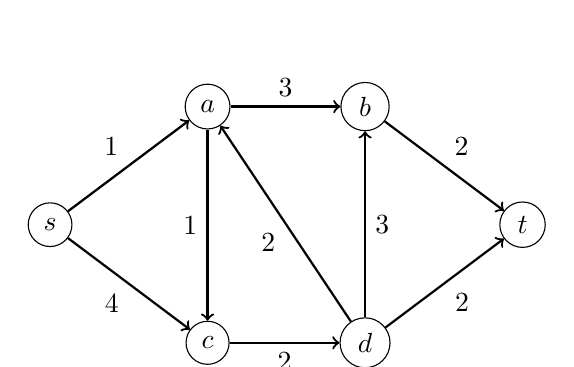
\begin{tikzpicture}
        \node[draw, circle] (s) at (0,0) {$s$};
        \node[draw, circle] (a) at (2,1.5) {$a$};
        \node[draw, circle] (b) at (4,1.5) {$b$};
        \node[draw, circle] (c) at (2,-1.5) {$c$};
        \node[draw, circle] (d) at (4,-1.5) {$d$};
        \node[draw, circle] (t) at (6,0) {$t$};

        \draw[thick, ->] (s) -- node[midway, anchor=south east]{$1$} (a);
        \draw[thick, ->] (s) -- node[midway, anchor=north east]{$4$} (c);
        \draw[thick, ->] (a) -- node[midway, anchor=south]{$3$} (b);
        \draw[thick, ->] (b) -- node[midway, anchor=south west]{$2$} (t);
        \draw[thick, ->] (c) -- node[midway, anchor=north]{$2$} (d);
        \draw[thick, ->] (d) -- node[midway, anchor=north west]{$2$} (t);
        \draw[thick, ->] (a) -- node[midway, anchor=east]{$1$} (c);
        \draw[thick, ->] (d) -- node[midway, anchor=north east]{$2$} (a);
        \draw[thick, ->] (d) -- node[midway, anchor=west]{$3$} (b);
    \end{tikzpicture}
    \caption{An example graph in which we want to calculate the flow from $s$ to $t$. On the edges we have the capacity of each edge}
    \label{fig:flow}
\end{figure}

First of all we see that the upper bound of the water going to $t$ is the sum of the capacities of the pipes going into $t$.

Then, to calculate if the solution is optimal or not we could partition the graph starting from $s$ and check how much water is flowing out of each partition.
This is a loose definition of \emph{cut}, but we will define it better later.

\subsubsection{Example: borrowing and lending}

Imagine there is a group of friends that could lend and borrow money from each other.
Each edge has an associated value that represent the \say{level of trust}, that is, how much money is $a$ willing to lend to $b$.

Assume that person $t$ wants to borrow from $s$. What is the maximum about $t$ will be able to borrow?

\subsection{Formal definitions}

\begin{definition}[$\delta^+(u)$ and $\delta^-(u)$]
    For a given directed graph $G = (V, E)$, let $u \in V$. Then we define
    \begin{align}
        \delta^+(u) & = \{(w, v) \in E : w = u\} \label{eq:flow:delta_plus}  \\
        \delta^-(u) & = \{(w, v) \in E : v = u\} \label{eq:flow:delta_minus}
    \end{align}
    that is, $\delta^+(u)$ is the set of edges outgoing from $u$, and $\delta^-(u)$ is the set of edges incoming in $u$.
\end{definition}

\begin{definition}[flow]
    \label{def:flow:flow}
    Let $G = (V, E)$ be a directed graph, and $s,t \in V$.
    A function $f:E \to \R^+$ is called a $s$-$t$ flow if it has the following proprieties:
    \begin{enumerate}[label=\roman*.]
        \item $f(a) \geq 0 \enspace \forall e \in E$
        \item $\sum_{e \in \delta^-(u)} f(e) = \sum_{e \in \delta^+(u)} f(e) \enspace \forall u \in V \setminus \{ s, t \}$, that is the flow that comes in is the same that goes out for every node other than $s$ and $t$.
    \end{enumerate}
\end{definition}

\begin{definition}[value of the flow]
    The value of an $s$-$t$ flow is defined as \begin{equation}
        {\operatorfont val} (f) = \sum_{e \in \delta^+(s)} f(e) - \sum_{e \in \delta^-(s)} f(e)
    \end{equation}
\end{definition}

\begin{remark}
    The following definition of value of flow is also equivalent:
    \begin{equation}
        {\operatorfont val} (f) = \sum_{e \in \delta^-(t)} f(e) - \sum_{e \in \delta^+(t)} f(e)
    \end{equation}
\end{remark}

\begin{definition}(capacity constraint)
    \label{def:flow:capacity_constraint}
    Let $c: E \to \R^+$ be a capacity function and $f$ a flow.
    We say that $f$ respects $c$ if $f(a)\leq c(a) \enspace \forall e \in E$.
\end{definition}

\begin{definition}[cut]
    Let $G = (V, E)$ be a directed graph.
    A cut is a partition of $V$ of the form $(U, V \setminus U)$.
    We will refer to the cut as $U$, since once $U$ and $V$ are given we can get the partition.
\end{definition}

\begin{definition}[$s$-$t$ cut]
    An $s$-$t$ cut is a cut $U$ such that $s \in U$ and $t \notin U$.
\end{definition}

\begin{definition}[capacity of a cut]
    The capacity if a cut $U$ is the amount of capacity on the edges that are going out of $U$.
    That is
    \begin{equation}
        {\operatorfont cap}(U) = \sum_{\substack{(w, v) \in E \\ w \in U \\ v \notin U}} c(w, v)
    \end{equation}
\end{definition}

\begin{remark}
    We extend the notation of $\delta^+$ and $\delta^-$ to cuts:
    \begin{align}
        \delta^+(U) & = \{(w, v) \in E : w \in U u, v \notin U\} \\
        \delta^-(U) & = \{(w, v) \in E : w \notin U u, v \in U\}
    \end{align}

    Note that if $U$ consists of just one element, then we get exactly \autoref{eq:flow:delta_plus} and \autoref{eq:flow:delta_minus}.
\end{remark}

\subsection{Algorithm}

\begin{definition}[maximum flow problem]
    Given a directed graph $G(V, E)$, $s, t \in V$, and a capacity function $c$ find an $s$-$t$ flow respecting $c$ of maximum value.
\end{definition}

\subsubsection{Proof of correctness}

\begin{theorem}[upper bound of the value of a flow]
    For any $s$-$t$ flow $f$ respecting $c$ and for any $s$-$t$ cut $U$ it holds that ${\operatorfont val}(f) \leq {\operatorfont cap}(U)$.
\end{theorem}

\begin{proof}
    We can rewrite the definition of value as
    \begin{align}
        {\operatorfont val}(f) & = \sum_{e \in \delta^+(s)} f(e) - \sum_{e \in \delta^-(s)} f(e)                                                                                                                                                       \\
                               & = \sum_{e \in \delta^+(s)} f(e) - \sum_{e \in \delta^-(s)} f(e) + \sum_{v \in U \setminus \{s\}} \underbrace{\left( \sum_{e \in \delta^+(v)} f(e) - \sum_{e \in \delta^-(v)} f(e)\right)}_{0} \label{eq:flow:proof_1} \\
                               & = \sum_{v \in U} \left( \sum_{e \in \delta^+(v)} f(e) - \sum_{e \in \delta^-(v)} f(e)\right)  \label{eq:flow:proof_2}                                                                                                 \\
                               & = \sum_{e \in \delta^+(U)} f(e) - \sum_{e \in \delta^-(U)} f(e) \label{eq:flow:proof_3}
    \end{align}
    where in \autoref{eq:flow:proof_1} we added the net flow which we know is $0$ by \autoref{def:flow:flow},
    in \autoref{eq:flow:proof_2} we added $s$ back in,
    and in \autoref{eq:flow:proof_3} we noted that if an edges $e \in U$, then


    Now by \autoref{def:flow:capacity_constraint} we note that
    \begin{equation}
        \sum_{e \in \delta^+(U)} f(e) \leq \sum_{e \in \delta^+(U)} c(e) = {\operatorfont cap}(U)
    \end{equation}

    Moreover by \autoref{def:flow:flow} we have that
    \begin{equation}
        \sum_{e \in \delta^-(U)} f(e) \geq 0
    \end{equation}

    Therefore
    \begin{equation}
        {\operatorfont val}(U) \leq \sum_{e \in \delta^+(U)} f(e) - \sum_{e \in \delta^-(U)} f(e) \leq {\operatorfont cap}(U)
    \end{equation}

\end{proof}

\subsubsection{Code}

The idea is to start with a flow of $0$. Then we start iterating and at each iteration we increase the value of the flow by checking if there are paths with some residual capacity.
We will be able to do this efficiently by using cuts.

An idea of an algorithm could be the following, note that it will NOT work as if we were to choose the wrong path we would get an incorrect result.

\begin{minted}{python}
    def flow(G, s, t, c):
        # Initialize the flow with 0
        f = {}
        for e in G.edges():
            f[e] = 0

        while True:
            # Construct a graph with the edges with some
            # residual capacity
            E = []
            for e in G.edges():
                if c(e) - f(e) > 0:
                    E.append(e)
            D = Graph(G.vertices(), E)

            # Find a path from s to t
            P = find_path(s, t, D)

            # If such path does not exist we stop
            if P is None:
                break

            # Find the edge of minimum capacity
            epsilon = min(
                P.edges(),
                key=lambda e_i: c(e_i) - f(e_i)
            )

            # Update the flow of all the edges in the path by
            # adding the minimum
            for e_i in P.edges:
                f[e_i] = f[e_i] + epsilon
\end{minted}

\subsubsection{Time complexity}

\end{document}